\subsection {Session 10, Exercise 10}

\lineparagraph {Exercise}

We are given two $0-1$ sequences, one of length $n$ and one of length $m$. The sequences are $a_1,a_2,\dots{},a_n$ and $b_1,b_2,\dots{},b_m$. Based on them an array $T$ is filled up as follows:

\begin{itemize}
    \item If $0\leq{}i\leq{}n$, then $T[i,0] = 0$.
    \item If $0\leq{}j\leq{}m$, then $T[0,j] = 0$.
    \item If $1\leq{}i\leq{}n$ and $1\leq{}j\leq{}m$, then
\end{itemize}

\begin{align*}
T[i,j] =
\begin{cases}
T[i-1, j-1] + 1 & \text{if } a_i = b_j \\
max(T[i,j-1], T[i-1,j]) & \text{if } a_i \neq{} b_j
\end{cases}
\end{align*}

What is the meaning of $T[i,j]$? What property of the two sequences is given by value $T[n,m]$?

\lineparagraph {Solution}

\begin{itemize}
\item Let's visualise this!
\end{itemize}

\begin{center}
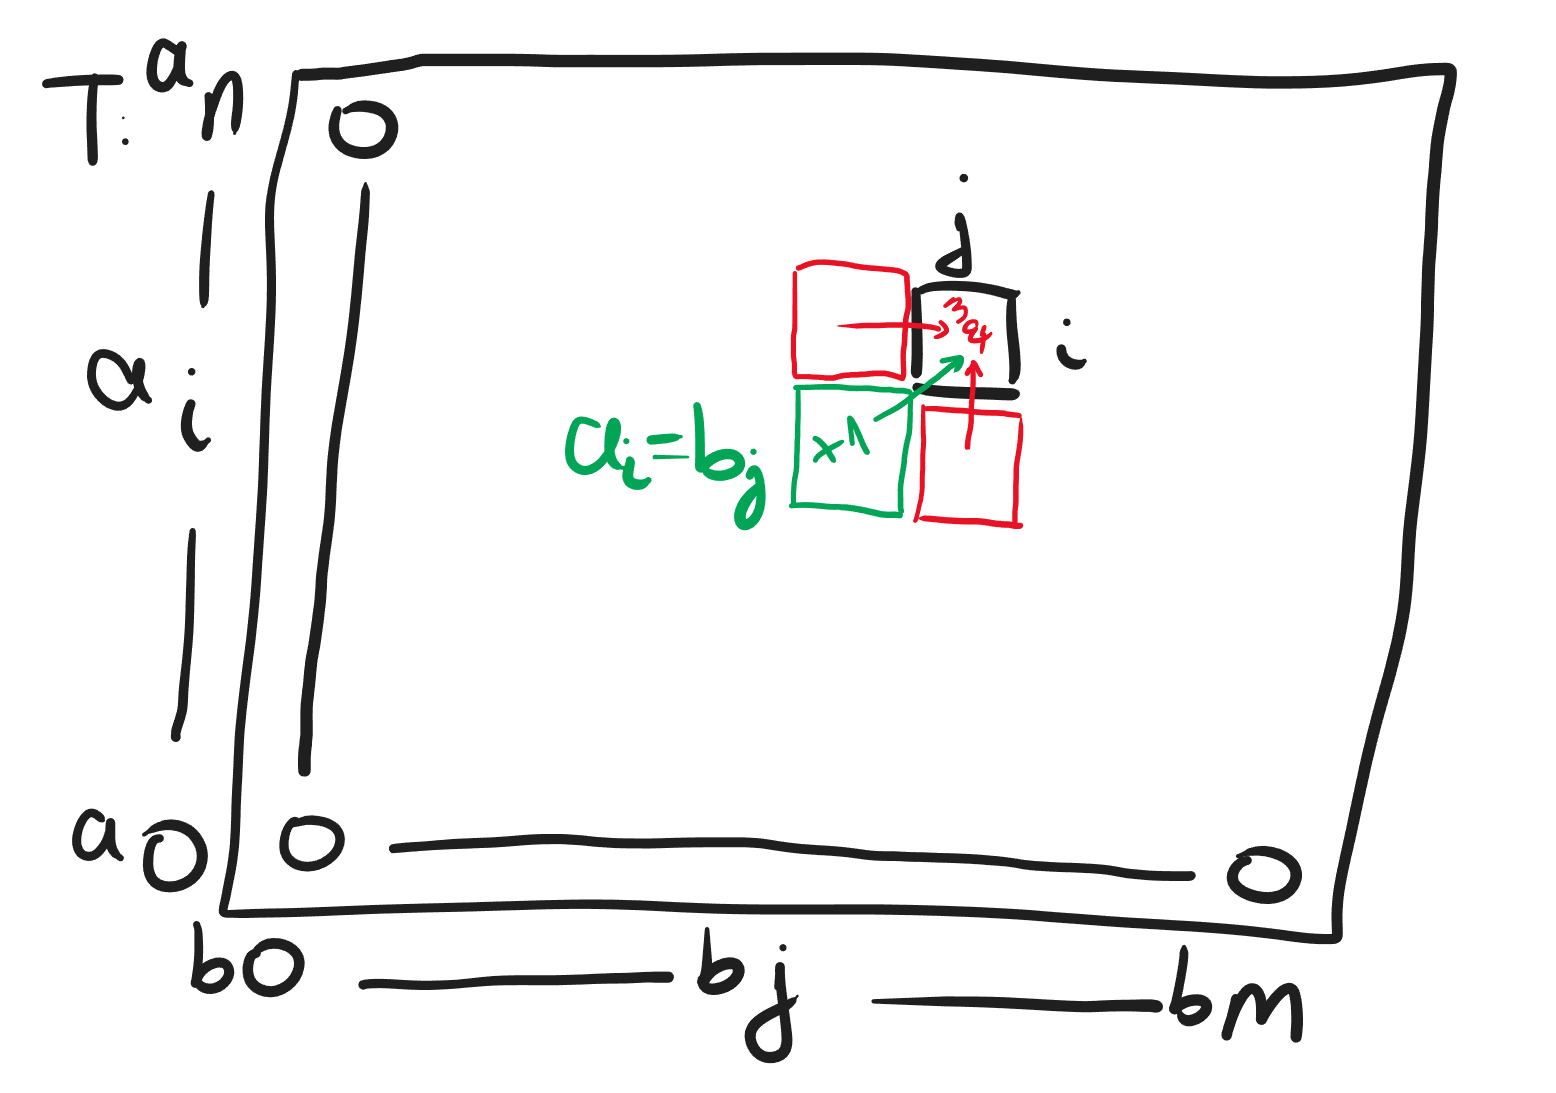
\includegraphics[width=\linewidth]{10/10/t_visualise.png}
\end{center}

\begin{itemize}
\item So we zero out all borders of the array, which is an alternative to having to give base cases: when we would be indexing out of the array, there is a border of zeroes that protects us and just returns a neutral element instead.
\item Then, in the formula, if $a_i = b_j$, that is very similar to the previous exercise, \nameref{session_10_exercise_9}: we count the matching characters with the $+1$ and add how many characters matched previously, with $T[i-1, j-1]$.
\item However, there is an alternative case: if the characters don't match, we take $T[i,j-1]$ or $T[i-1,j]$, whichever is bigger. This means that we are allowed to skip over non-matching characters from either side: the matching sequence does not have to be from \textbf{consecutive} characters, but could be any \textbf{non-consecutive} subsequence from $a$ and $b$.
\item So $T[n,m]$ contains the length of the longest, not necessarily consecutive subsequences that are the same from $a$ and $b$. And $T[i,j]$ does the same, but for he prefix $a_1\dots{}a_i$ and $b_1\dots{}b_j$.
\end{itemize}